\documentclass[11pt,a4paper]{article}

\usepackage[margin=2.2cm]{geometry}
\usepackage[T1]{fontenc}
\usepackage{lmodern}
\usepackage{microtype}
\usepackage{amsmath,amssymb}
\usepackage{booktabs}
\usepackage{tabularx}
\usepackage{array}
\usepackage{xurl}
\usepackage{enumitem}
\usepackage{graphicx}
\usepackage{pdflscape}
\usepackage{xcolor}
\usepackage{tikz}
\newcommand{\step}[1]{\tikz[baseline=(c.base)]\node[draw,circle,inner sep=0.6pt,minimum size=1.15em,font=\scriptsize](c){#1};}
\usepackage[colorlinks=true,linkcolor=blue!50!black,urlcolor=blue!50!black,citecolor=blue!50!black]{hyperref}

\graphicspath{{../../diagrams/}}
\setlist{itemsep=2pt,topsep=4pt}
\renewcommand{\arraystretch}{1.25}
\renewcommand{\topfraction}{0.9}
\renewcommand{\textfraction}{0.08}
\renewcommand{\floatpagefraction}{0.8}
\newcolumntype{L}{>{\raggedright\arraybackslash}X}
\newcolumntype{P}[1]{>{\raggedright\arraybackslash}p{#1}}

\title{\textbf{Metis-Auto v2}\\[2pt]\large A measured LLM router built on UniRoute}
\author{Proposal v2 \quad\textbullet\quad Rahnema College 2026}
\date{19 October 2026}

\begin{document}
\maketitle

\begin{abstract}
\noindent Chatbot platforms pay very different prices for different AI models, while many messages
are simple. The course asks for a router that picks a cheap model when that is enough and a strong
model when it is not, without sacrificing quality. We build the router exactly as in UniRoute
(Jitkrittum et al., ICLR 2026), following our specification \texttt{UNIROUTE\_PIPELINE.md}: a large
\emph{unlabeled} set of real prompts is grouped into $K$ clusters; each candidate model answers a small
labeled validation set, graded by an LLM judge checked against humans; each model's fail rate per
cluster becomes its fingerprint; and each new message goes to the model with the lowest fail rate plus
$\lambda\times$cost in its cluster. New models are added without retraining. The router sits inside a
gateway with hard rules, a semantic cache, failover, escalation and traces. We wait for the full
dataset before any paid API call. Estimated API cost: \textbf{\$17--50} (\textbf{\$60} planned),
recomputed from the full data first.
\end{abstract}

%=====================================================================
\section{Why version 2}

Version 1 (17 October) used the 377 sample turns for everything: clustering, report cards, choosing
settings and the final numbers. Comparing it with the paper and our pipeline specification showed
three problems.

\medskip
\noindent\begin{tabularx}{\linewidth}{@{}P{70mm} L@{}}
\toprule
\textbf{Problem in v1} & \textbf{Fix in v2} \\
\midrule
Clusters and report cards came from the \emph{same} labeled data, which overfits & Clusters from a large \emph{unlabeled} train split; report cards only from the validation split \\
$K$ and $\lambda$ were tuned on the same data we reported on & A \textbf{locked test set}, used once at the end \\
Answers were graded against production's answer, which came from 18 different models & Pointwise grading, or pairwise against a fixed \emph{anchor} model, chosen by a \textbf{pilot} \\
\bottomrule
\end{tabularx}

\medskip
\noindent The paper's setting needs thousands of unlabeled prompts and about 700 labeled ones; only
the full dataset can provide that.

%=====================================================================
\section{Problem}

\noindent\begin{tabularx}{\linewidth}{@{}P{58mm} L@{}}
\toprule
\textbf{Need (course brief, dataset)} & \textbf{Why it is hard} \\
\midrule
Users should not choose models (``AI decision fatigue'') & The system must judge each message automatically and cheaply \\
Cut cost without hurting quality & Quality is easy to claim and hard to measure \\
Mostly Persian traffic & Judges and routers are checked mainly in English; we found no router research on Persian \\
Four very different usage types & The design must generalize, not be tuned to one chatbot \\
Reliability and observability & Provider outages and rate limits; every decision must be explainable \\
\bottomrule
\end{tabularx}

%=====================================================================
\section{Solution overview}

The \textbf{offline build} (specification steps S1--S12) splits the data, clusters the unlabeled train
split, generates and grades answers on the validation and test splits, computes fingerprints, chooses
$K$ and $\lambda$, evaluates once on the test split and packages a versioned \textbf{router artifact}.
The \textbf{online gateway} applies hard rules, embeds the message, checks the semantic cache, routes
with UniRoute, calls the model with failover, runs code checks with escalation, and records a trace
(Figure~\ref{fig:overview}).

\begin{figure}[!htbp]
\centering
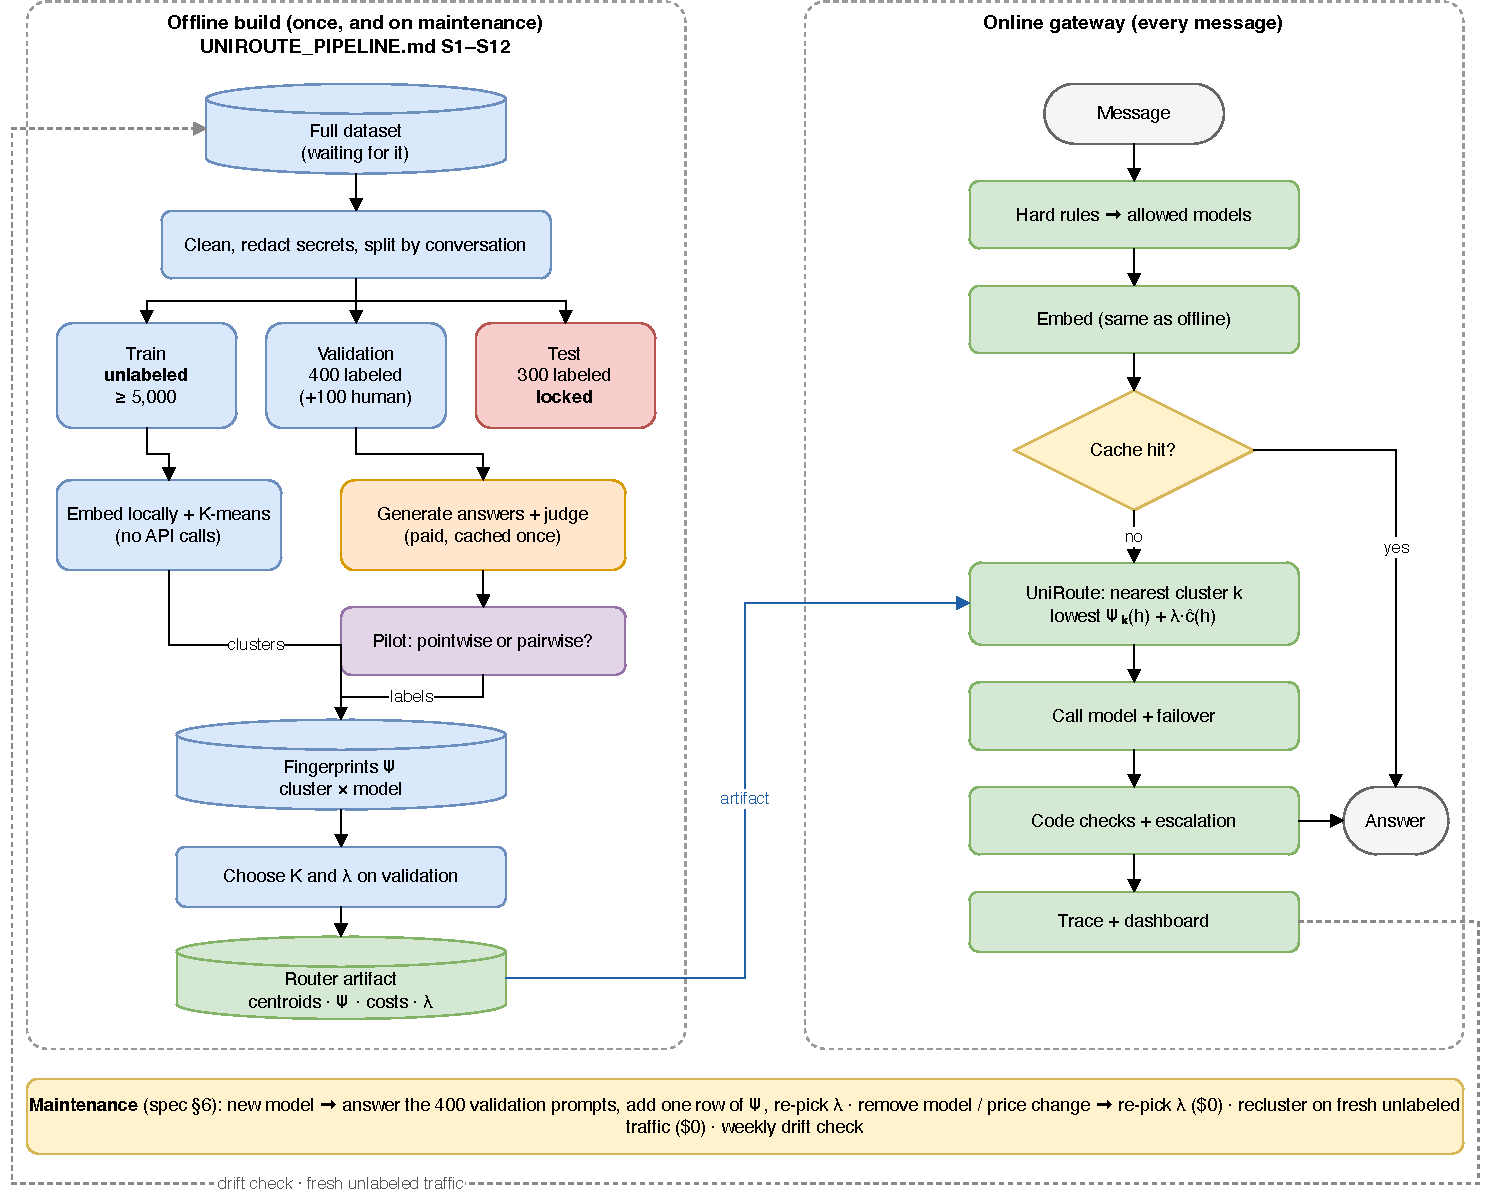
\includegraphics[width=0.95\linewidth]{01-overview.pdf}
\caption{Offline build, online gateway, and maintenance.}
\label{fig:overview}
\end{figure}

%=====================================================================
\section{How UniRoute works}\label{sec:uniroute}

Figure~\ref{fig:uniroute} shows every UniRoute step on one page. The step codes (S1--S12, R1--R4,
M1--M4) match the specification; a full walkthrough is in \texttt{docs/uniroute-explained.md}.

\noindent\begin{tabularx}{\linewidth}{@{}P{31mm} P{17mm} L@{}}
\toprule
\textbf{Band} & \textbf{Steps} & \textbf{What happens} \\
\midrule
1 Prepare & S1, S2, S3 & Clean prompts (last message + 2 turns); split by conversation into \textbf{train (unlabeled)}, validation 400, test 300 (locked); register models, anchor and costs $\hat c(h)\in[0,1]$ \\
2 Prompt types (free) & S4, S5 & Embed the train prompts with a local multilingual model; K-means finds $K$ clusters (centroids) without labels \\
3 Fingerprints (paid) & S6, S7, S8 & Every model answers validation and test once; the judge turns each answer into a loss (pointwise or pairwise, chosen by the pilot); $\Psi_k(h)$ = model $h$'s average loss on the validation prompts of cluster $k$ \\
4 Settings & S9, S10 & $K$ by split-validation; $\lambda$ for a quality target or a cost budget; validation only \\
5 Evaluate and ship & S11, S12 & One evaluation on the locked test set against always-best, always-cheapest, ZeroRouter and K-NN; a versioned router artifact \\
6 Route (online) & R1--R4 & Embed, find the nearest cluster $k^{*}$, score $s(h)=\Psi_{k^{*}}(h)+\lambda\,\hat c(h)$, route to the lowest (fallback: next lowest) \\
7 Maintain & M1--M4 & Add a model (one new row of $\Psi$), remove a model, price change, traffic drift; \textbf{no retraining} \\
\bottomrule
\end{tabularx}

\paragraph{Worked example} (specification, Appendix B; $\lambda=0.4$).

\medskip
\noindent\begin{tabularx}{\linewidth}{@{}P{30mm} L L L P{16mm}@{}}
\toprule
\textbf{Prompt type} & \textbf{S (strong, anchor)} & \textbf{M (medium)} & \textbf{C (cheap)} & \textbf{Route to} \\
\midrule
Casual chat & $0.50+0.40=0.90$ & $0.52+0.12=0.64$ & $0.55+0.02=\mathbf{0.57}$ & \textbf{C} \\
Persian literature & $0.50+0.40=\mathbf{0.90}$ & $0.80+0.12=0.92$ & $0.92+0.02=0.94$ & \textbf{S} \\
\bottomrule
\end{tabularx}

\medskip
\noindent In chat the cheap model is almost as good as the anchor and 20 times cheaper, so it wins. In
literature its loss is much higher, so paying for S is worth it. With $\lambda=0$ the router always
picks S; with a very large $\lambda$ it always picks C.

\begin{landscape}
\begin{figure}[p]
\centering
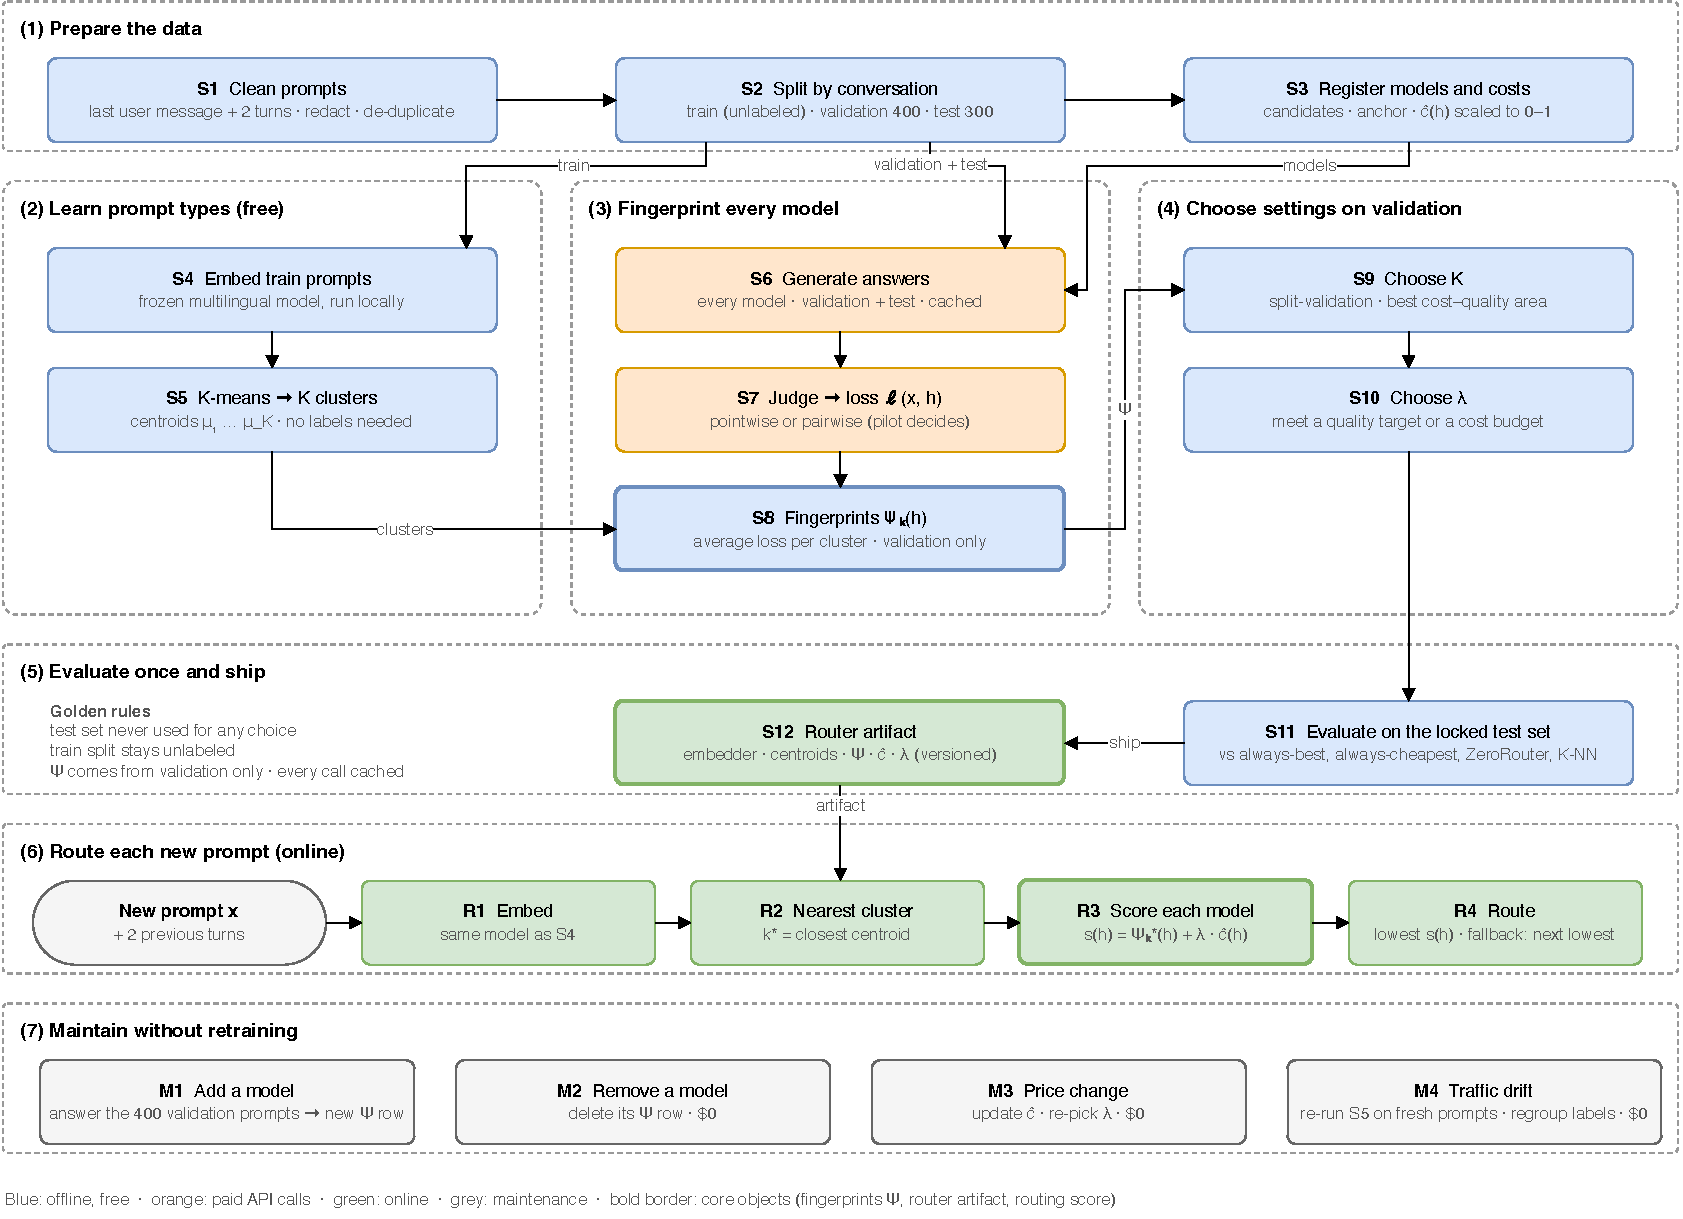
\includegraphics[width=\linewidth,height=0.86\textheight,keepaspectratio]{05-uniroute.pdf}
\caption{UniRoute, every step (S1--S12 offline, R1--R4 online, M1--M4 maintenance). Blue: offline and free; orange: paid API calls; green: online; grey: maintenance; bold border: core objects (fingerprints $\Psi$, router artifact, routing score).}
\label{fig:uniroute}
\end{figure}
\end{landscape}

%=====================================================================
\section{Offline build}

\begin{figure}[!htbp]
\centering
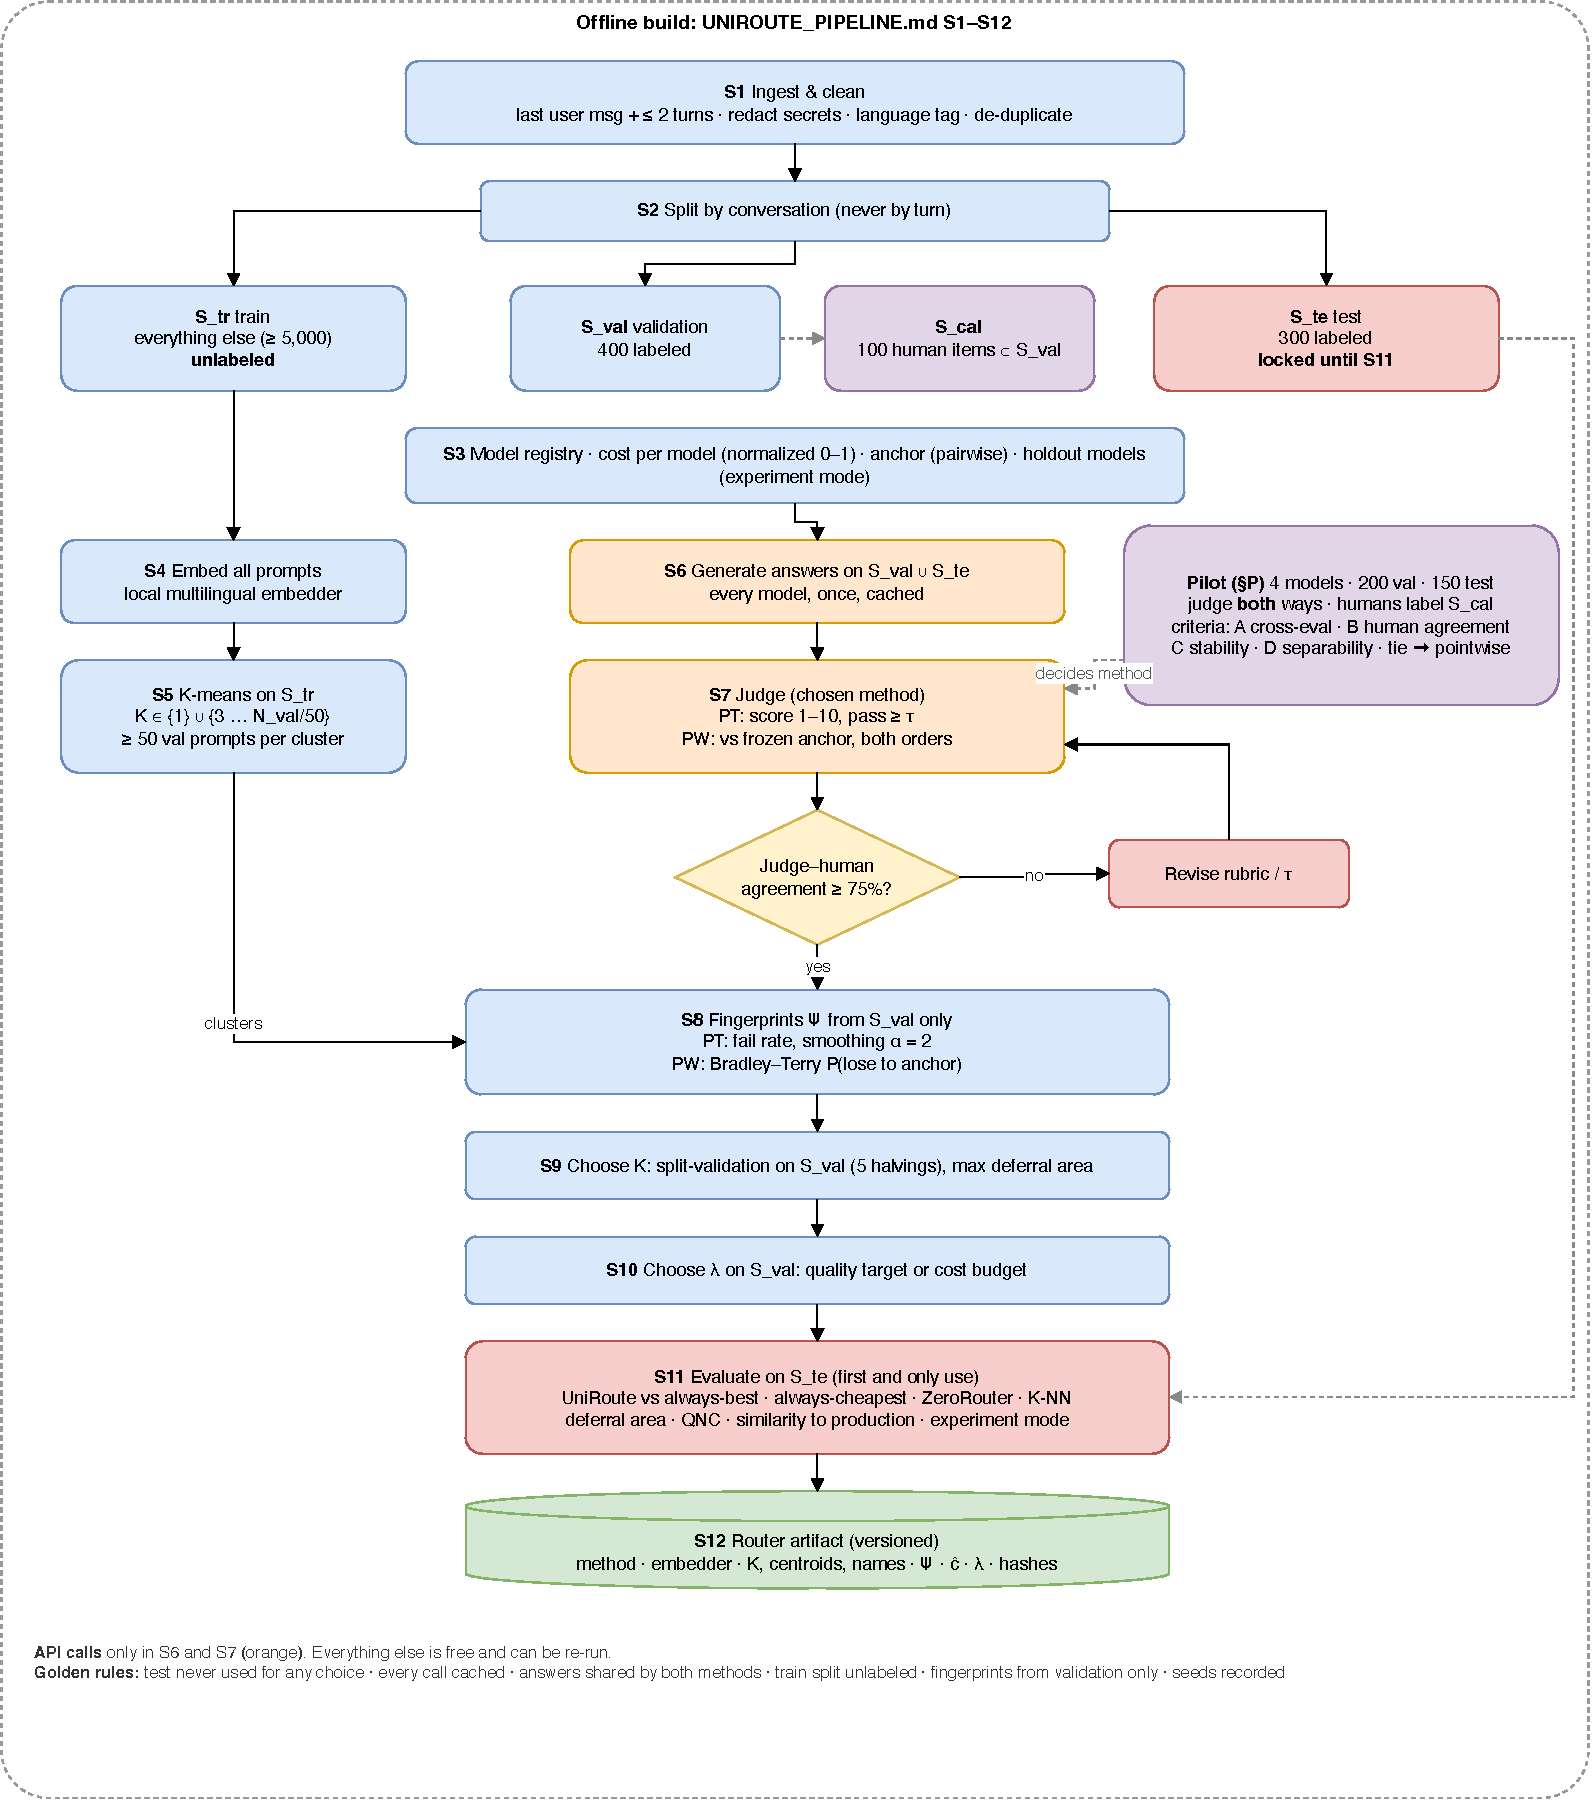
\includegraphics[width=\linewidth,height=0.78\textheight,keepaspectratio]{02-offline-build.pdf}
\caption{Offline build (S1--S12). Only S6 and S7 make paid API calls.}
\label{fig:offline}
\end{figure}

\noindent\begin{tabularx}{\linewidth}{@{}P{28mm} L P{12mm}@{}}
\toprule
\textbf{Step} & \textbf{What} & \textbf{API} \\
\midrule
S1 Clean & Routable prompt = last user message + up to 2 earlier turns; redact secrets; language tag; de-duplicate & 0 \\
S2 Split & By conversation: train (unlabeled, ideally $\ge$ 5{,}000), validation 400, test 300 (locked), calibration 100 $\subset$ validation & 0 \\
S3 Models & 5 candidates; cost per model from real token counts, normalized to $[0,1]$; anchor = strongest & 0 \\
S4--S5 Cluster & Local multilingual embedder; K-means on train for $K\in\{3,\dots,\lfloor N_{\text{val}}/50\rfloor\}$ plus $K=1$; $\ge$ 50 validation prompts per cluster & 0 \\
S6 Generate & Every model answers validation and test once, with its chatbot's own system prompt and context; cached & paid \\
S7 Judge & Pointwise (score 1--10, pass if $\ge\tau$) or pairwise against the anchor (both orders); judge--human agreement $\ge$ 75\% & paid \\
S8 Fingerprints & Fail rate per cluster with smoothing $\alpha=2$ ($\alpha=0$ is the paper's eq.~12), or Bradley--Terry $P(\text{lose to anchor})$ & 0 \\
S9--S10 Settings & $K$ by split-validation on the validation set; $\lambda$ for a quality target or a cost budget & 0 \\
S11 Evaluate & On the locked test set only (Section~\ref{sec:eval}) & 0 \\
S12 Package & Router artifact: embedder, centroids, cluster names, fingerprints, costs, $\lambda$ & 0 \\
\bottomrule
\end{tabularx}

\medskip
\noindent{\raggedright\textbf{Candidate models (5):} \texttt{gemini-2.5-flash-lite}, \texttt{deepseek-v4-flash},
\texttt{gpt-4o-mini}, \texttt{gemini-2.5-flash}, \texttt{claude-sonnet-4-6} (strong; anchor).
\textbf{Judge:} a strong Persian-capable model outside the pool, temperature 0, blind to model names.\par}

\paragraph{The pilot.} Before the full build we run a pilot on part of the full data: 4 models, 200
validation and 150 test prompts, \emph{both} grading methods on the same answers, and 100 human labels.
It picks the method by (A) routing quality under both measures, (B) agreement with humans,
(C) stability of the fingerprints and (D) whether the labels can tell models apart. Ties go to
pointwise, which is cheaper. Everything the pilot pays for is reused.

\paragraph{Routing rule} (paper eq.~8 and 11). For a message $x$ in cluster $k(x)$:
\[
  r(x) \;=\; \arg\min_{h}\; \Psi_{k(x)}(h) + \lambda\cdot\hat c(h),
\]
where $\Psi_k(h)$ is model $h$'s fail rate (or loss against the anchor) in cluster $k$ and $\hat c(h)$
is its normalized cost.

%=====================================================================
\section{Online gateway}

\begin{figure}[!htbp]
\centering
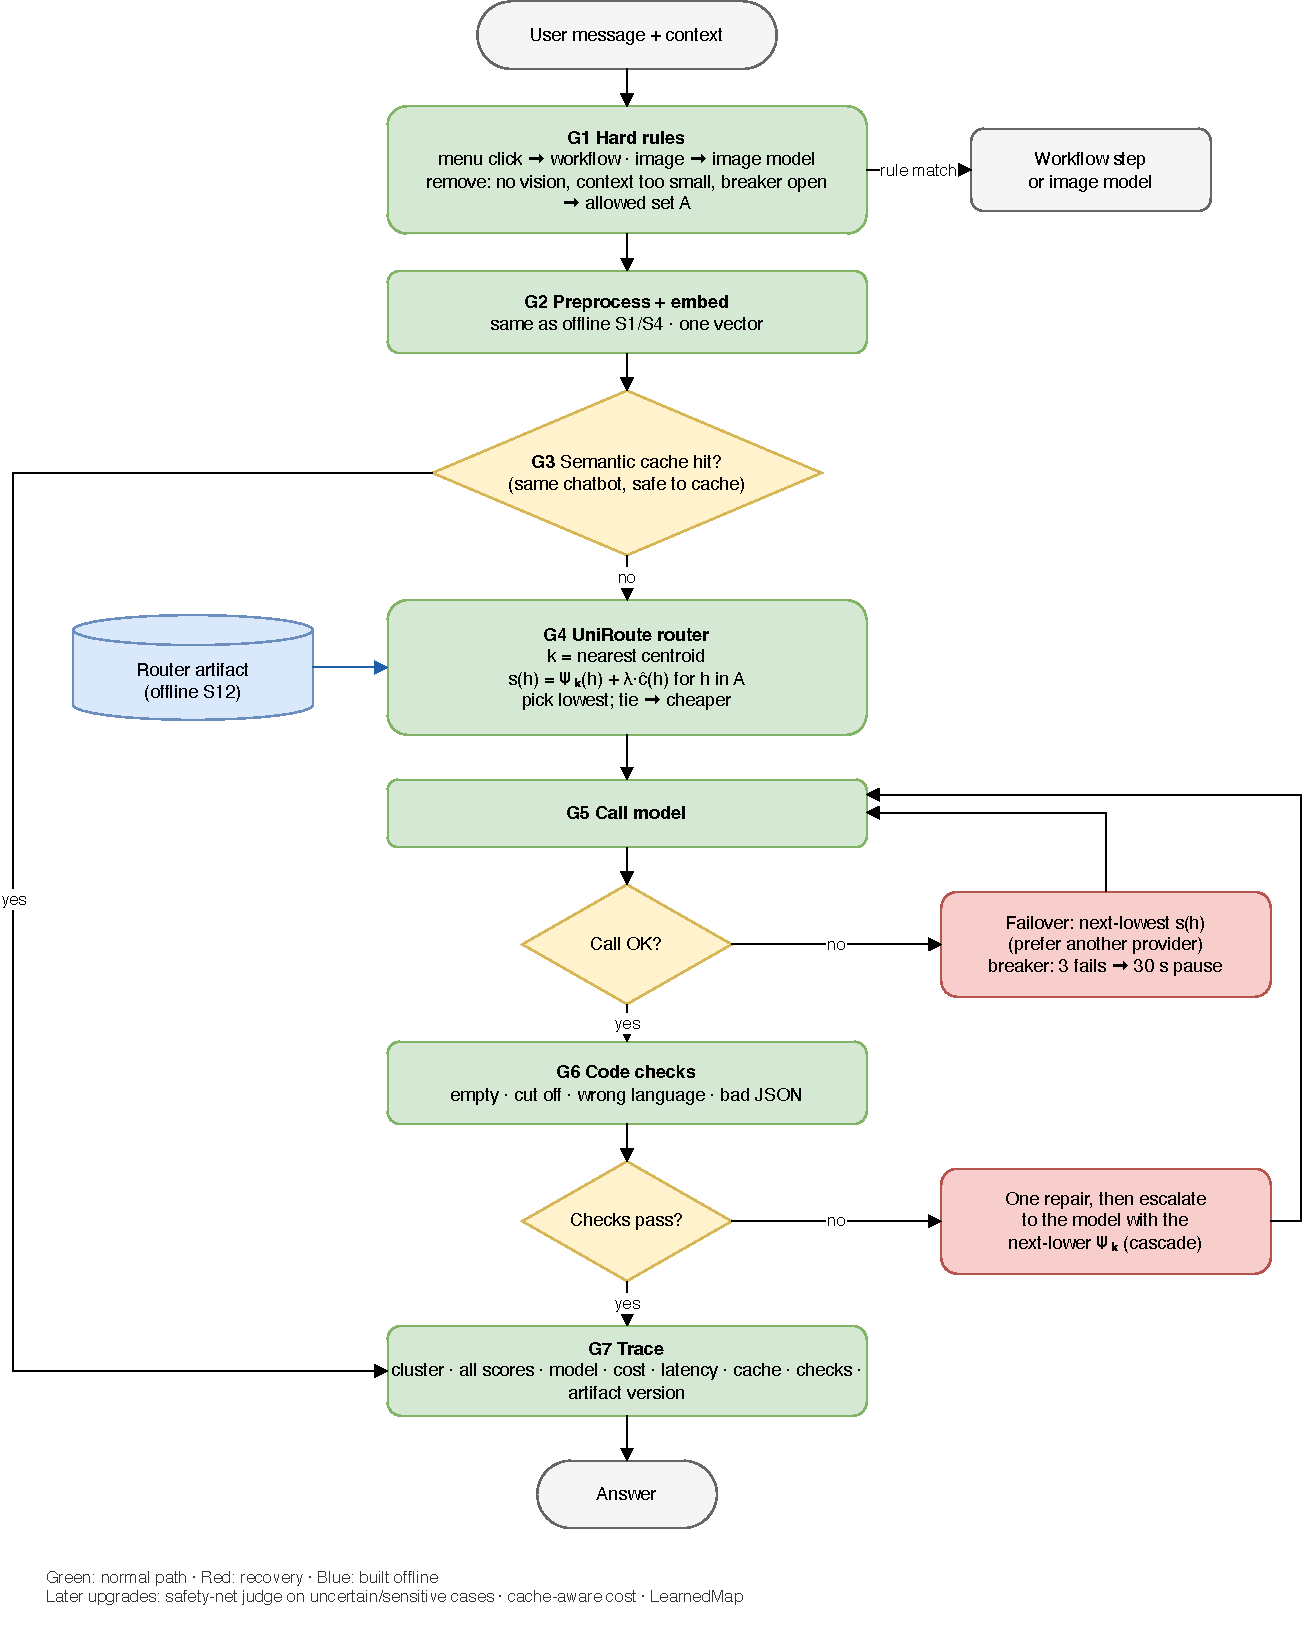
\includegraphics[height=0.72\textheight]{03-online-path.pdf}
\caption{Online path for one message. Red boxes are recovery steps.}
\label{fig:online}
\end{figure}

\noindent\begin{tabularx}{\linewidth}{@{}P{26mm} L@{}}
\toprule
\textbf{Stage} & \textbf{What it does} \\
\midrule
G1 Hard rules & Menu clicks go to the workflow step, images to the image model; remove models without vision, with too small a context window, or with an open circuit breaker \\
G2 Embed & Same preprocessing and embedder as offline; one vector \\
G3 Cache & Same chatbot and language only; never follow-ups, personal or sensitive content; threshold for $\le$ 2\% false hits \\
G4 Router & Nearest cluster; lowest $\Psi_k(h)+\lambda\hat c(h)$ among the allowed models \\
G5 Call & On error, the next-lowest score, preferably another provider; circuit breaker (3 failures, then a 30\,s pause) \\
G6 Checks & Free code checks (empty, cut off, wrong language, bad JSON), one repair, then escalate to the next-lower-loss model (the brief's cascade) \\
G7 Trace & Cluster, all scores, model, cost, latency, cache hit, checks, artifact version \\
\bottomrule
\end{tabularx}

%=====================================================================
\section{Evaluation}\label{sec:eval}

All results come from the \textbf{locked test set}, used once.

\medskip
\noindent\begin{tabularx}{\linewidth}{@{}P{42mm} L@{}}
\toprule
\textbf{Strategy} & \textbf{What it is} \\
\midrule
Always-best & The strongest model for everything (the brief's premium baseline) \\
Always-cheapest & The cheapest model for everything \\
ZeroRouter & No clusters; mixes the two best-value models (paper's baseline) \\
K-NN & Uses the most similar validation prompts (paper's baseline) \\
\textbf{UniRoute (K-means)} & Our router \\
Production & Cost and similarity only (what actually happened) \\
\bottomrule
\end{tabularx}

\medskip
\noindent\textbf{Metrics:} area under the cost--quality (deferral) curve; QNC, the lowest cost at
which routing matches the best single model; cost saved at equal quality; quality per cluster and per
category; routing share per model; semantic similarity to production's answers (the brief's metric);
cost per 1{,}000 queries; p50/p90 latency; cache hit rate.

\paragraph{Simulating new models.} We hide about a third of the models while choosing $K$ and
$\lambda$, then route only among them. This tests UniRoute's main claim.

\paragraph{Overfitting checks (all free).} Locked test set; $K$ by split-validation; $K=1$ baseline;
fingerprint stability; separability; validation-versus-test gap.

\paragraph{Success criteria.}
\begin{itemize}
  \item UniRoute's curve area $\ge$ ZeroRouter's and K-NN's on the test set.
  \item At least 40\% cheaper than always-best at no more than 2 points lower quality.
  \item p90 latency no worse than always-best.
  \item Every number labeled measured or simulated, with confidence intervals.
\end{itemize}

\noindent\textbf{Honest framing:} with a fixed set of models the paper finds UniRoute only about as
good as simpler routers (its App.~G.5). Its advantage is adding models without retraining. We report
the comparison either way.

%=====================================================================
\section{Plan and budget}

\begin{figure}[!htbp]
\centering
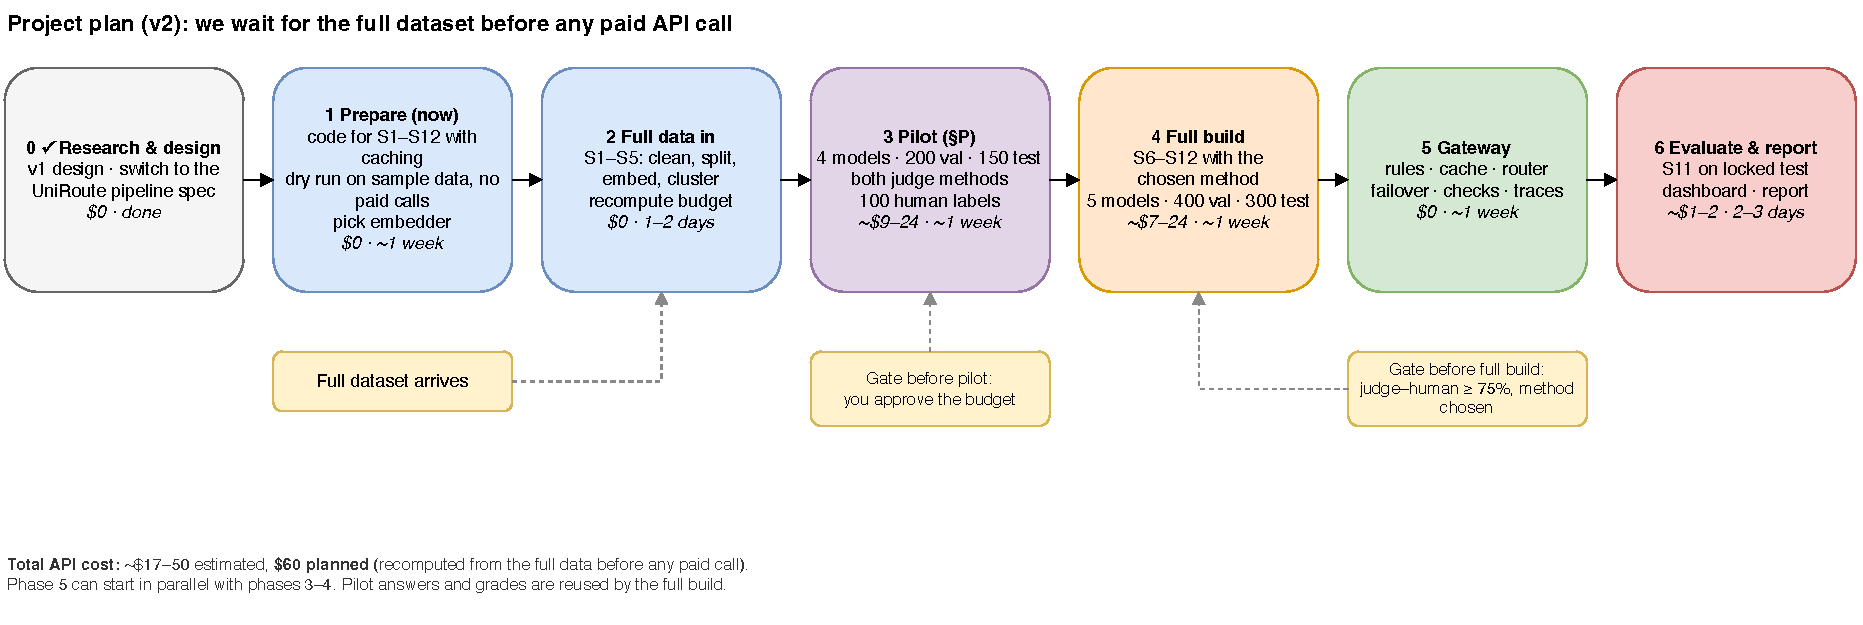
\includegraphics[width=\linewidth]{04-plan.pdf}
\caption{Project phases. No paid API call happens before the full dataset arrives.}
\label{fig:plan}
\end{figure}

\noindent\begin{tabularx}{\linewidth}{@{}P{10mm} L P{20mm} P{20mm}@{}}
\toprule
\textbf{Phase} & \textbf{What} & \textbf{API cost} & \textbf{Time} \\
\midrule
0 \checkmark & Research, v1 design, switch to the UniRoute pipeline specification & \$0 & done \\
1 & Now, while waiting: code for S1--S12 with caching; dry run on the sample data with no paid calls; choose the embedder & \$0 & $\sim$1 week \\
2 & Full data arrives: S1--S5; recompute the budget & \$0 & 1--2 days \\
3 & Pilot: 4 models, 200 val, 150 test, both grading methods, 100 human labels & $\sim$\$9--24 & $\sim$1 week \\
4 & Full build S6--S12 with the chosen method: 5 models, 400 val, 300 test & $\sim$\$7--24 & $\sim$1 week \\
5 & Gateway: rules, cache, router, failover, checks, traces (can overlap 3--4) & \$0 & $\sim$1 week \\
6 & Evaluate on the locked test set; dashboard; report & $\sim$\$1--2 & 2--3 days \\
\midrule
\textbf{Total} & & \textbf{\$17--50 (plan \$60)} & \textbf{4--5 weeks after the data} \\
\bottomrule
\end{tabularx}

\paragraph{Gates.} The team approves the recomputed budget before the pilot; the judge must agree with
humans at least 75\% of the time before the full build.

\begin{figure}[!htbp]
\centering
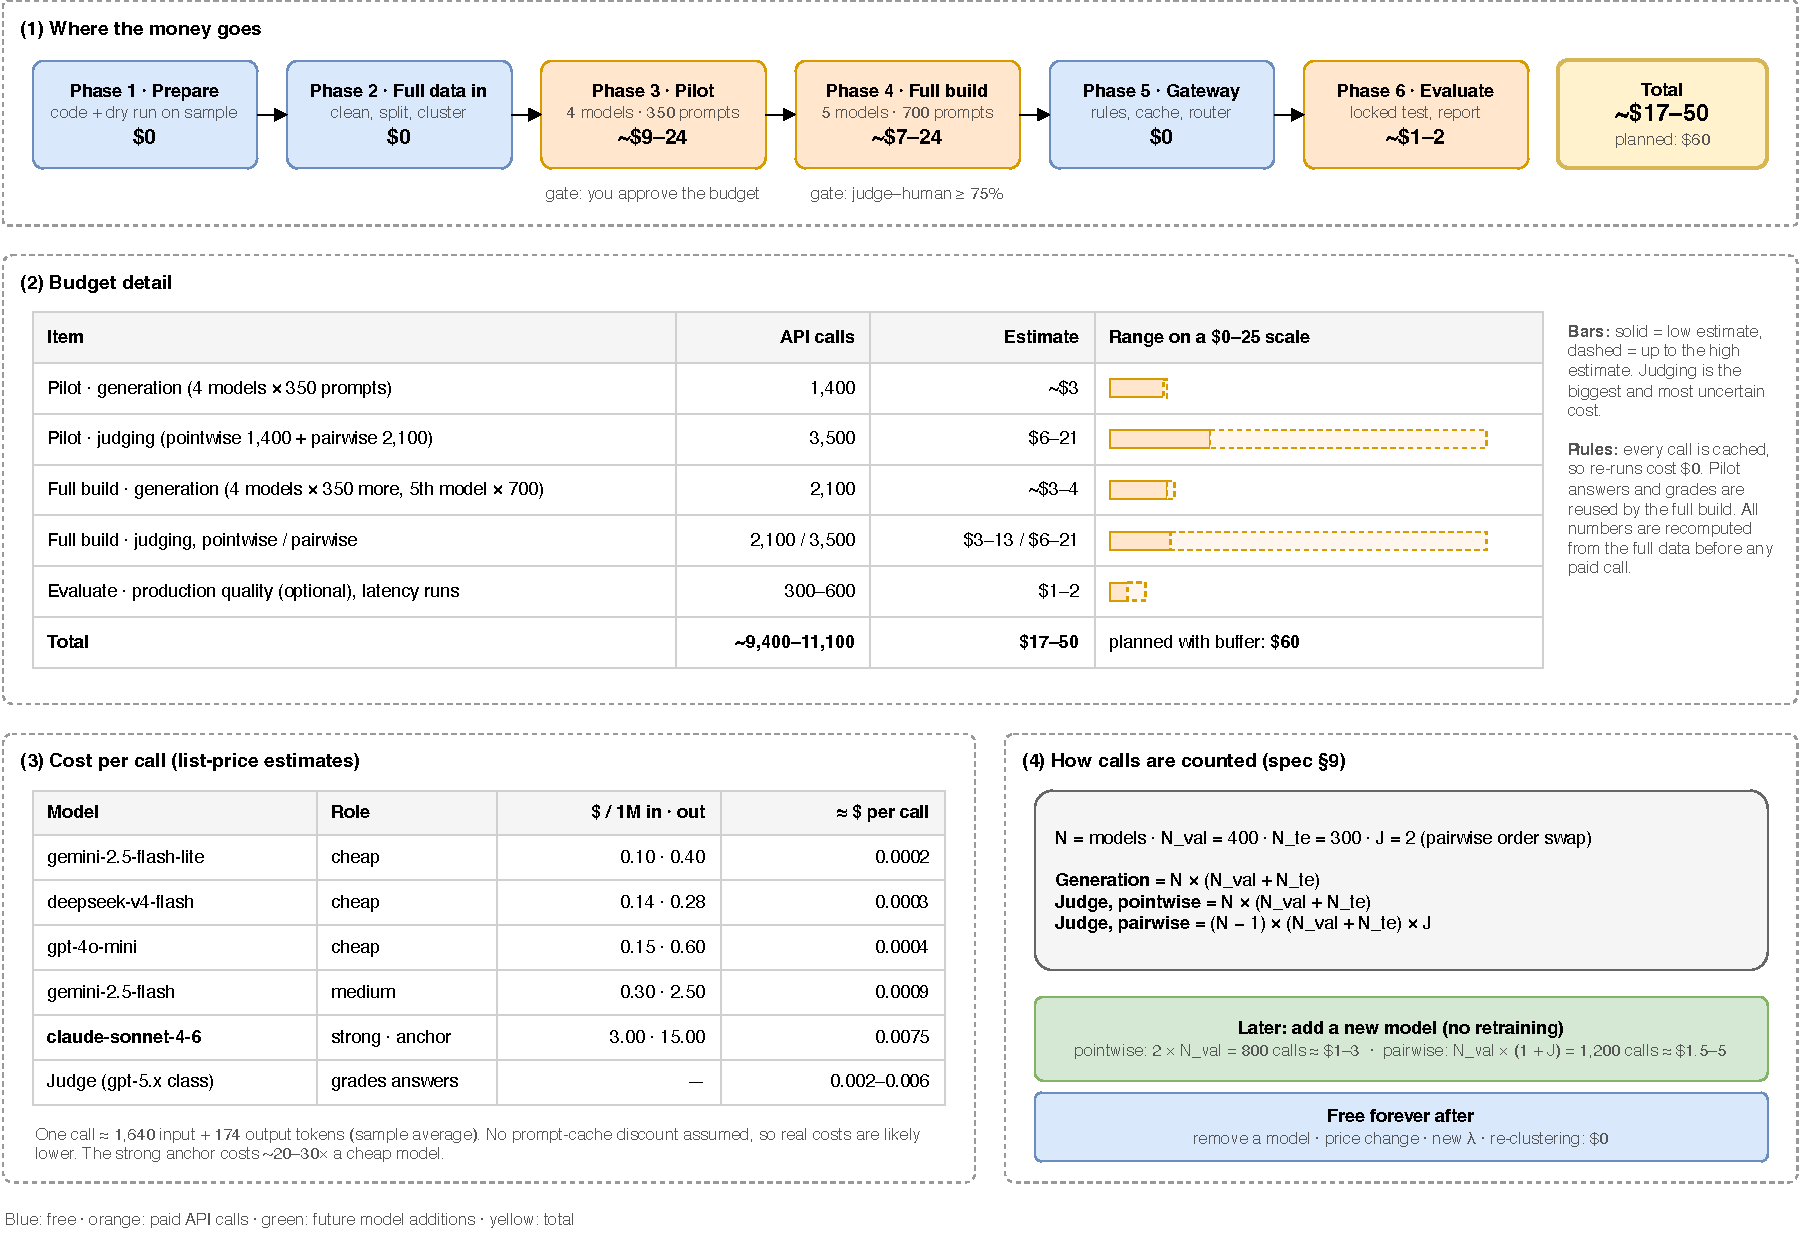
\includegraphics[width=\linewidth]{06-api-costs.pdf}
\caption{API costs: where the money goes, budget detail with low--high ranges, cost per call, and how calls are counted. Every call is cached, so re-runs cost \$0.}
\label{fig:costs}
\end{figure}

\medskip
\noindent\begin{tabularx}{\linewidth}{@{}L P{22mm} P{27mm}@{}}
\toprule
\textbf{Budget item} & \textbf{Calls} & \textbf{Estimate} \\
\midrule
Pilot generation (3 cheap models + anchor, 350 prompts) & 1{,}400 & $\sim$\$3 \\
Pilot judging (pointwise 1{,}400 + pairwise 2{,}100) & 3{,}500 & \$6--21 \\
Full-build generation (extra prompts, 5th model) & $\sim$2{,}100 & \$3--4 \\
Full-build judging, pointwise / pairwise & $\sim$2{,}100 / 3{,}500 & \$3--13 / \$6--21 \\[-2pt]
Production quality on test (optional), live latency runs & 300--600 & \$1--2 \\
\midrule
\textbf{Total} & & \textbf{\$17--50} \\
\bottomrule
\end{tabularx}

\medskip
\noindent Per-call prices come from the sample's token counts ($\sim$1{,}640 input and $\sim$174
output tokens per turn) and list prices; a judge call costs about \$0.002--0.006. All estimates are
recomputed from the full data before any paid call.

\subsection*{Later upgrades}

\noindent\begin{tabularx}{\linewidth}{@{}P{58mm} L@{}}
\toprule
\textbf{Upgrade} & \textbf{Why} \\
\midrule
LearnedMap (paper \S5.2) & Soft cluster assignment; needs labels for 3--5 models on a few thousand train prompts \\
Safety-net judge on uncertain or sensitive messages & Extra protection where clusters are unsure \\
Cache-aware cost per message & Staying with one provider is cheaper thanks to prompt caching \\
Attribute-based clusters (paper App.~G.4) & More robust when traffic changes \\
2--3 answers per (prompt, model); a second judge & Less noisy labels (DARS, EMNLP 2026) \\
Shared cache and breaker state (Redis) & Several gateway instances \\
\bottomrule
\end{tabularx}

%=====================================================================
\section{Risks}

\noindent\begin{tabularx}{\linewidth}{@{}P{62mm} L@{}}
\toprule
\textbf{Risk} & \textbf{Mitigation} \\
\midrule
Full dataset late or smaller than needed & Phase 1 is useful regardless; with less data, smaller validation/test sets and fewer clusters, stated in the report \\
Judge unreliable in Persian & Human agreement gate $\ge$ 75\%; pilot criterion B \\
Labels cannot tell models apart & Pilot criterion D; raise $\tau$ or switch to pairwise \\
UniRoute no better than simpler routers & Reported honestly; keep the winner in the gateway \\
Only 5 models weakens the new-model test & Optionally add 1--3 candidates \\
Estimated prices & Recompute before any paid call \\
Credentials in the dataset & Redact before any API call; never commit data or generated answers \\
\bottomrule
\end{tabularx}

%=====================================================================
\section{Decisions needed}

\begin{enumerate}
  \item \textbf{Full dataset:} when does it arrive, and how large is it?
  \item \textbf{API access:} OpenRouter, direct provider keys, AvalAI, or Google Cloud?
  \item \textbf{Budget:} approve about \$60 in principle (final number after the full data arrives).
  \item \textbf{Human calibration:} who labels 100 Persian answers in the pilot?
  \item \textbf{Candidate pool:} keep 5 models, or add 1--3 for a stronger new-model test?
  \item \textbf{Ask the course team} what the \texttt{default} model in the data means.
  \item \textbf{Deadline and deliverable format.}
\end{enumerate}

%=====================================================================
\section*{References}
\begin{enumerate}[label={[\arabic*]}]
  \item Jitkrittum et al. Universal Model Routing for Efficient LLM Inference (UniRoute). ICLR 2026. \url{https://arxiv.org/abs/2502.08773} --- primary research
  \item Hu et al. RouterBench (ZeroRouter and K-NN baselines). 2024. \url{https://arxiv.org/abs/2403.12031}
  \item From Sampled Outcomes to Capability Distributions (DARS). EMNLP 2026. \url{https://arxiv.org/abs/2606.06924}
  \item Dynamic Model Routing and Cascading for Efficient LLM Inference: A Survey. 2026. \url{https://arxiv.org/abs/2603.04445}
  \item How Reliable is Multilingual LLM-as-a-Judge? EMNLP 2025 Findings. \url{https://aclanthology.org/2025.findings-emnlp.587/}
  \item RouterArena. ICLR 2026. \url{https://arxiv.org/abs/2510.00202}
\end{enumerate}

\end{document}
